% =========================================================
%  2026夏季学期《计算机系统综合实践Ⅰ》实验报告
%  编译方式：xelatex（需编译两遍以生成目录）
%    xelatex main.tex && xelatex main.tex
%  或直接：make
% =========================================================
\documentclass[UTF8,a4paper,12pt,fontset=none]{ctexart}

% =========================================================
% 0. 报告信息（在此修改）
% =========================================================
\newcommand{\ReportTitle}{2026夏季学期《计算机系统综合实践Ⅰ》实验报告}
\newcommand{\ReportHeaderTitle}{《计算机系统综合实践Ⅰ》实验报告}
\newcommand{\StudentName}{彭湘莲}
\newcommand{\StudentID}{24020007096}
\newcommand{\StudentTerm}{2026夏季学期}
\newcommand{\ReportDate}{2026年9月}

% =========================================================
% 1. 字体设置（严格按照格式要求）
%    论文标题：黑体，四号；正文：宋体，小四；
%    英文及数字：Times New Roman，小四
% =========================================================
\setmainfont{Times New Roman}                 % 英文与数字
\setCJKmainfont{SimSun}[                      % 正文中文：宋体
  BoldFont=SimHei,
  ItalicFont=KaiTi
]
\setCJKsansfont{SimHei}
\setCJKmonofont{FangSong}[ItalicFont=KaiTi]
\setCJKfamilyfont{zhsong}{SimSun}
\setCJKfamilyfont{zhhei}{SimHei}
\setCJKfamilyfont{zhkai}{KaiTi}
\setCJKfamilyfont{zhfs}{FangSong}
\newcommand{\songti}{\CJKfamily{zhsong}}
\newcommand{\heiti}{\CJKfamily{zhhei}}
\newcommand{\kaishu}{\CJKfamily{zhkai}}
\newcommand{\fangsong}{\CJKfamily{zhfs}}

% =========================================================
% 2. 常用宏包
% =========================================================
\usepackage{amsmath,amssymb}
\usepackage{array,booktabs,tabularx,multirow}
\usepackage{caption,float,graphicx,subcaption}
\usepackage{enumitem}
\usepackage{etoolbox}
\usepackage{fancyhdr}
\usepackage{geometry}
\usepackage{hyperref}
\usepackage{listings}
\usepackage{setspace}
\usepackage{tikz}
\usepackage{xcolor}

\usetikzlibrary{arrows.meta,calc,fit,positioning,shapes.geometric}

% =========================================================
% 3. 页面设置（A4 电子版）
% =========================================================
\geometry{a4paper,top=2.7cm,bottom=2.5cm,left=2.6cm,right=2.6cm}
\setlength{\headheight}{26pt}
\onehalfspacing

\definecolor{oucblue}{RGB}{0,84,158}
\definecolor{ouclight}{RGB}{235,245,255}
\definecolor{codebg}{RGB}{248,249,251}
\definecolor{codecomment}{RGB}{0,120,80}
\definecolor{codekeyword}{RGB}{0,72,160}
\definecolor{codestring}{RGB}{170,70,30}

\hypersetup{
  colorlinks=true,
  linkcolor=oucblue,
  citecolor=oucblue,
  urlcolor=oucblue,
  pdftitle={\ReportTitle},
  pdfauthor={\StudentName}
}

% 图注、表注：宋体五号，英文与数字 Times New Roman；标签加粗
\DeclareCaptionFont{capfont}{\zihao{5}}
\captionsetup{font=capfont,labelfont={capfont,bf},labelsep=quad}
% 表格内文字：宋体五号、单倍行距，英文与数字 Times New Roman
\AtBeginEnvironment{tabular}{\zihao{5}\singlespacing}
\AtBeginEnvironment{tabularx}{\zihao{5}\singlespacing}
\numberwithin{figure}{section}
\numberwithin{table}{section}
\renewcommand{\thefigure}{\thesection-\arabic{figure}}
\renewcommand{\thetable}{\thesection-\arabic{table}}
\setlist{itemsep=0.1em,topsep=0.4em,parsep=0.1em}
\AtBeginEnvironment{itemize}{\singlespacing}

% =========================================================
% 4. 标题格式：章标题（黑体四号，居中，"第X章"编号）；
%    节标题：黑体小四（目录与书签自动同步"第X章"）
% =========================================================
\ctexset{
  section = {
    name        = {第,章},
    number      = \arabic{section},
    format      = \centering\heiti\zihao{4},
    aftername   = \quad,
    beforeskip  = 1.6em plus .3ex,
    afterskip   = 1.0em,
  },
  subsection = {
    format      = \heiti\zihao{-4},
    aftername   = \quad,
    beforeskip  = 1.2em plus .2ex,
    afterskip   = 0.6em,
  }
}

% =========================================================
% 5. 页眉页脚（正文开始启用，页号从第 1 页起）
%    页眉：题目；页脚：姓名 学号 页号
% =========================================================
\newcommand{\HeaderLogo}{%
  \IfFileExists{assets/ouc-logo.png}
    {
\includegraphics[height=0.68cm]{assets/ouc-logo.png}}
    {\textcolor{oucblue}{\bfseries OUC}}%
}

\fancypagestyle{main}{
  \fancyhf{}
  \fancyhead[L]{\HeaderLogo}
  \fancyhead[R]{\small\ReportHeaderTitle}
  \fancyfoot[C]{\small\StudentName-\StudentID-第\thepage 页}
  \renewcommand{\headrulewidth}{0.4pt}
  \renewcommand{\footrulewidth}{0pt}
}

% =========================================================
% 6. 代码样式
% =========================================================
\lstdefinestyle{reportcode}{
  basicstyle=\ttfamily\small,
  keywordstyle=\color{codekeyword}\bfseries,
  commentstyle=\color{codecomment}\itshape,
  stringstyle=\color{codestring},
  backgroundcolor=\color{codebg},
  breaklines=true,
  columns=fullflexible,
  frame=single,
  framerule=0.5pt,
  rulecolor=\color{black!20},
  numbers=left,
  numberstyle=\tiny\color{black!50},
  numbersep=10pt,
  showstringspaces=false,
  tabsize=4,
  captionpos=b
}
\lstset{style=reportcode}

% 灰色提示文字：完成报告后替换或删除。
\newcommand{\placeholder}[1]{\textcolor{black!55}{\emph{#1}}}

% 设计图占位框：把图片放入 assets/ 后，用 \includegraphics 替换即可
\newcommand{\figplaceholder}[1]{%
  \fcolorbox{black!35}{black!3}{%
    \parbox[c][0.30\textheight][c]{0.88\linewidth}{%
      \centering\color{black!45}%
      {\large\heiti 设计图占位区}\\[0.5em]
      #1\\[0.5em]
      {\small 请将图片放入 \texttt{assets/}，用\\[0.3em]
       \texttt{\textbackslash includegraphics[width=0.9\textbackslash linewidth]\{assets/...\}} 插入}%
    }%
  }%
}

% 仿真波形占位框
\newcommand{\waveplaceholder}[1]{%
  \fcolorbox{black!35}{black!3}{%
    \parbox[c][0.16\textheight][c]{0.88\linewidth}{%
      \centering\color{black!45}%
      {\large\heiti 仿真波形占位区}\\[0.4em]
      #1\\[0.4em]
      {\small 插入仿真截图：\texttt{\textbackslash includegraphics[width=0.92\textbackslash linewidth]\{assets/...\}}}%
    }%
  }%
}

% =========================================================
% 7. 正文
% =========================================================
\begin{document}
\hypersetup{pageanchor=false}

% ---------------------------------------------------------
% 封面（无页眉页脚）
% ---------------------------------------------------------
\begin{titlepage}
  \centering
  \vspace*{1.0cm}

  % 校徽与校名
  \IfFileExists{assets/ouc-logo.png}{%
    
\includegraphics[width=0.28\linewidth]{assets/ouc-logo.png}\par
    \vspace{0.8cm}
    {\heiti\zihao{2}中国海洋大学\par}
  }{%
    \fbox{\parbox[c][3cm][c]{6cm}{\centering\Huge OUC}}\par
  }

  \vspace{2.8cm}

  % 题目
  {\heiti\zihao{2}《计算机系统综合实践Ⅰ》\par}
  \vspace{0.5cm}
  {\heiti\zihao{2}实验报告\par}

  \vspace{3.0cm}

  % 姓名、学号、学期（填空线样式）
  {\renewcommand{\arraystretch}{2.2}
    \begin{tabular}{r@{：}l}
      {\heiti\zihao{3}姓\hspace{1em}名} & \underline{\makebox[6.5cm][c]{\zihao{3}\StudentName}} \\
      {\heiti\zihao{3}学\hspace{1em}号} & \underline{\makebox[6.5cm][c]{\zihao{3}\StudentID}} \\
      {\heiti\zihao{3}学\hspace{1em}期} & \underline{\makebox[6.5cm][c]{\zihao{3}\StudentTerm}} \\
    \end{tabular}\par
  }

  \vfill
  {\zihao{4}\ReportDate\par}
  \vspace*{1.0cm}
  \thispagestyle{empty}
\end{titlepage}

% ---------------------------------------------------------
% 目录（自动生成，无页眉页脚）
% ---------------------------------------------------------
\clearpage
\pagestyle{empty}
\begingroup
  \makeatletter
  \linespread{1.25}\selectfont
  \begin{center}
    {\heiti\zihao{3}目\hspace{1.5em}录\par}
  \end{center}
  \vspace{0.4em}
  \setcounter{tocdepth}{2}
  \@starttoc{toc}
  \makeatother
\endgroup

% ---------------------------------------------------------
% 正文：页码从第 1 页开始，启用页眉页脚
% ---------------------------------------------------------
\clearpage
\pagenumbering{arabic}
\setcounter{page}{1}
\hypersetup{pageanchor=true}
\pagestyle{main}

% 论文标题（黑体，四号）
\begin{center}
  {\heiti\zihao{4}\ReportTitle\par}
\end{center}
\vspace{0.5em}

% =========================================================
\section{实验概述}
% =========================================================
\subsection{实验目的}

本实验以教材配套的 MiniMIPS32 处理器及实验工程为对象，通过阅读 RTL 代码、分析处理器结构并运行测试程序，理解五级流水线 RISC 处理器的工作过程。具体目的如下：

\begin{itemize}
  \item 熟悉 \textbf{MiniMIPS32 指令集}与处理器基本组成，理解各类指令在流水线中的执行过程；
  \item 掌握 \textbf{五级流水线}（IF、ID、EX、MEM、WB）及各流水段寄存器的作用；
  \item 理解 \textbf{数据相关与控制相关}的成因，掌握 \textbf{定向前推}、\textbf{转移处理}与\textbf{流水线暂停}机制；
  \item 理解 \textbf{CP0 与异常处理}机制，掌握异常检测、状态保存与 ERET 返回的过程；
  \item 熟悉 \textbf{Vivado 工程}，能结合测试程序与仿真波形分析处理器运行结果。
\end{itemize}

\subsection{实验内容}

实验围绕 MiniMIPS32 原型系统与处理器核两个层次展开，由系统结构到内部数据通路逐步深入。具体包括：

\begin{itemize}
  \item 分析 \textbf{MiniMIPS32\_SYS 原型系统总体结构}，明确处理器、存储器与外围接口的连接关系；
  \item 分析 \textbf{MiniMIPS32 处理器顶层结构}，掌握内部数据通路与主要模块；
  \item 分析 \textbf{五级流水线各段}及四个流水段寄存器的功能；
  \item 分析 \textbf{定向前推}、\textbf{转移指令处理}与\textbf{流水线暂停}机制；
  \item 分析 \textbf{CP0 与异常处理}机制，理解异常检测、状态保存与 ERET 返回过程；
  \item 结合测试程序完成 \textbf{功能仿真}，依据寄存器、PC、存储器及控制信号状态判断运行结果。
\end{itemize}

\subsection{实验环境与资料}

开发工具为 Vivado，硬件描述语言为 Verilog HDL，分析对象为 MiniMIPS32 五级流水线处理器及其顶层原型系统 MiniMIPS32\_SYS；RTL 代码与功能测试程序均由实验提供，参考资料为《计算机系统设计（上册）——基于 FPGA 的 RISC 处理器设计与实现》。

% =========================================================
\section{MiniMIPS32原型系统总体结构}
% =========================================================
\subsection{MiniMIPS32\_SYS总体结构}

MiniMIPS32\_SYS 是本次实验所分析的完整原型系统，在一块 FPGA 上集成了处理器、存储器和外设。系统由以下部件构成：核心是 MiniMIPS32 处理器；配套的指令存储器存放待执行的程序，数据存储器存放运行中的数据；外设包括单色 LED、RGB LED、七段数码管和 Timer，统一经 I/O 译码模块接入；处理器与存储器、外设之间的连接则由设备接口模块完成。系统总体结构如图 \ref{fig:sys-top} 所示。

外部输入的 100\,MHz 系统时钟，先由时钟模块分频为 50\,MHz，作为处理器和各模块的工作时钟。

从数据流角度看，处理器对外存在两条通路：一是\textbf{取指通路}，CPU 把当前 PC 作为地址送往指令存储器，取回下一条指令；二是\textbf{数据访存通路}，CPU 执行 Load、Store 指令时把数据地址送往设备接口，由设备接口根据地址把请求转发到数据存储器或 I/O 译码模块。存储器和外设采用\textbf{统一编址}，CPU 只需给出地址，具体访问哪一个部件由设备接口负责路由。

\begin{figure}[H]
  \centering
  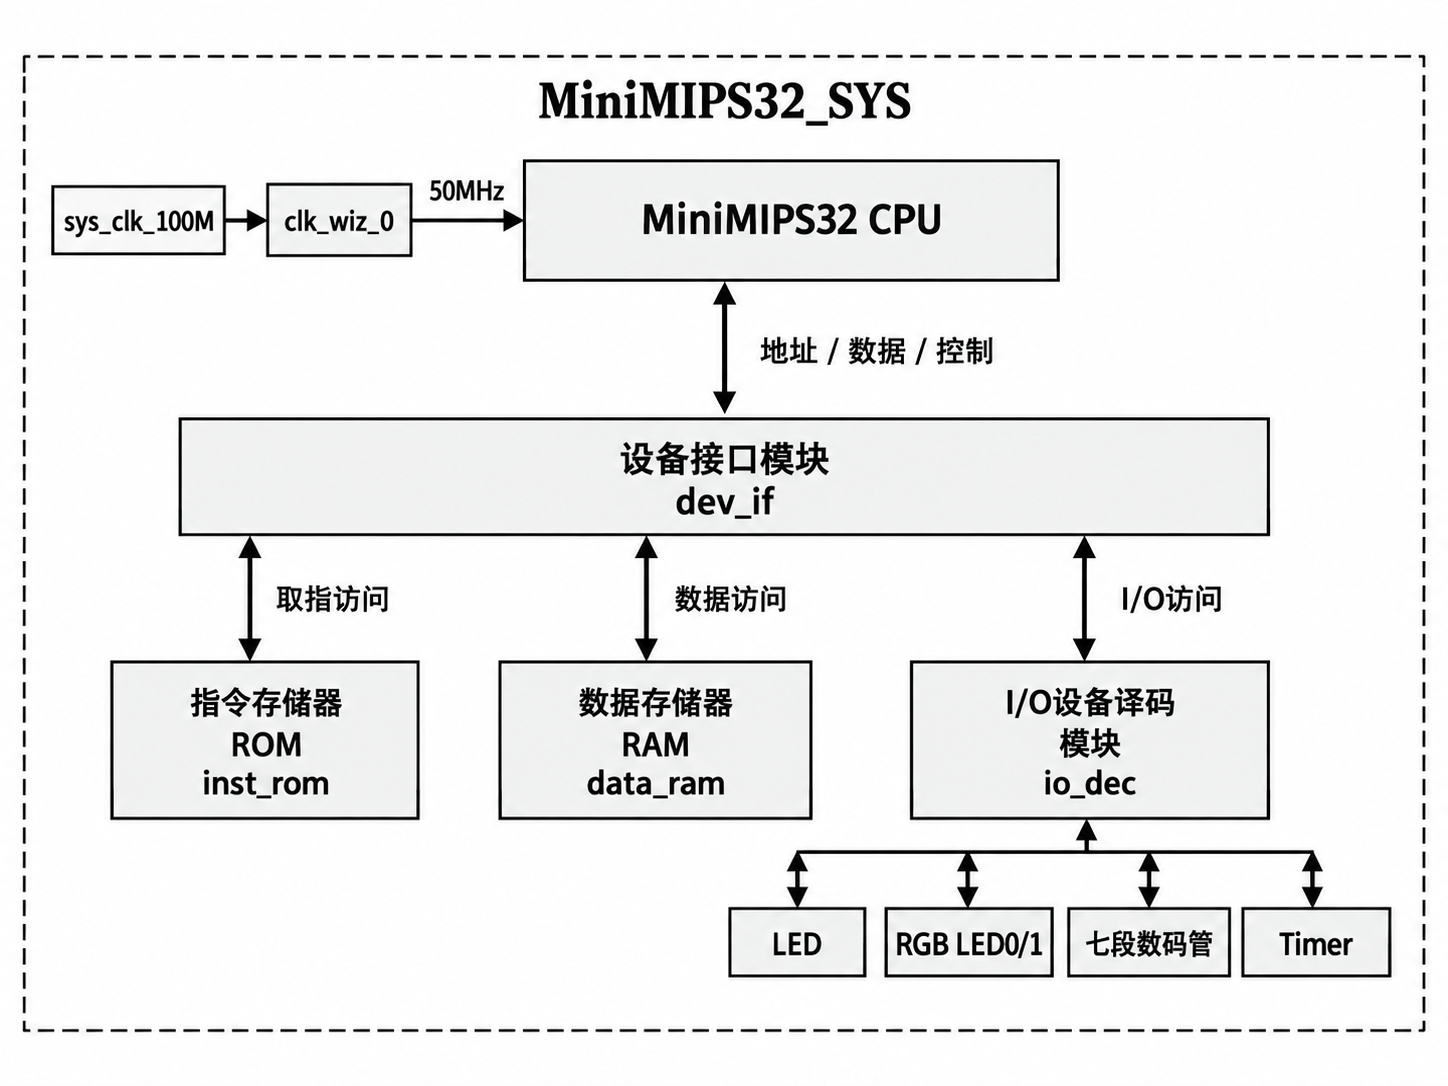
\includegraphics[width=0.92\linewidth]{assets/sys.png}
  \caption{MiniMIPS32\_SYS 系统硬件架构}
  \label{fig:sys-top}
\end{figure}

\subsection{主要模块及访问关系}

各主要模块的作用如表 \ref{tab:sys-mods} 所示。

\begin{table}[H]
  \centering
  \caption{MiniMIPS32\_SYS 主要模块}
  \label{tab:sys-mods}
  \begin{tabularx}{\linewidth}{llX}
    \toprule
    模块 & 对应模块名 & 主要作用 \\
    \midrule
    MiniMIPS32 处理器 & \texttt{MiniMIPS32} & 执行指令并产生取指、访存及相关控制信号 \\
    时钟模块 & \texttt{clk\_wiz\_0} & 将 100\,MHz 系统时钟转换为 50\,MHz 工作时钟 \\
    设备接口 & \texttt{dev\_if} & 完成 CPU 与 ROM、RAM 和 I/O 设备之间的访问选择及数据传递 \\
    指令存储器 & \texttt{inst\_rom} & 存放程序指令，根据取指地址输出 32 位指令 \\
    数据存储器 & \texttt{data\_ram} & 保存程序运行过程中的数据，完成数据读写 \\
    I/O 译码 & \texttt{io\_dec} & 对 I/O 地址进行译码，并完成 LED、RGB LED、七段数码管和 Timer 的控制 \\
    \bottomrule
  \end{tabularx}
\end{table}

处理器内部采用五级流水线，对外只暴露取指和数据两组接口：取指接口给出指令地址并接收指令，数据接口给出地址、写数据与读写使能并接收读回数据，其内部结构将在第 3、4 章分析。

设备接口负责两类请求的路由与转发。对取指请求，它将指令地址与片选信号送往指令存储器，并把读回的指令返回 CPU；对数据请求，则依据地址判断访问目标。工程约定，数据地址高 16 位为 \texttt{0xBFD0} 时属于 I/O 空间，判定条件为

\[
\text{daddr}[31{:}16] = \text{0xBFD0}
\]

满足该条件的访问送往 I/O 译码模块，其余送往数据存储器。读数据时，设备接口同样按地址从数据存储器或 I/O 译码模块中选择一路数据返回 CPU，从而实现存储器和外设的统一编址访问。

指令存储器存放程序指令，CPU 按 PC 取指；数据存储器存放运行数据，供 LB、LH、LW、SB、SH、SW 等访存指令读写。I/O 译码模块收到设备接口转发的请求后，再按地址低 16 位选择具体外设，各外设的地址分配如表 \ref{tab:io-addr} 所示。

\begin{table}[H]
  \centering
  \caption{I/O 设备地址分配}
  \label{tab:io-addr}
  \begin{tabularx}{\linewidth}{llX}
    \toprule
    I/O 设备 & 完整地址 & 功能 \\
    \midrule
    单色 LED & \texttt{0xBFD0F000} & 16 位 LED 输出 \\
    RGB LED0 & \texttt{0xBFD0F100} & RGB LED0 输出 \\
    RGB LED1 & \texttt{0xBFD0F104} & RGB LED1 输出 \\
    七段数码管 & \texttt{0xBFD0F200} & 显示 32 位数据 \\
    Timer & \texttt{0xBFD0E000} & 32 位计数器读写 \\
    \bottomrule
  \end{tabularx}
\end{table}

单色 LED、RGB LED 和七段数码管作为输出设备使用；Timer 在 I/O 译码模块内部以 32 位寄存器实现，随时钟递增，可通过地址 \texttt{0xBFD0E000} 读写。处理器虽预留了外部中断输入，但本工程顶层将该输入固定为 \texttt{6'b0}，故 Timer 不作为 CPU 的外部中断源使用。

% =========================================================
\section{MiniMIPS32处理器总体架构}
% =========================================================
\subsection{支持的指令集}
\placeholder{列出并分类本处理器支持的 56 条指令，说明各指令格式（R/I/J 型）
与编码字段，建议用表格。}

\begin{table}[H]
  \centering
  \caption{支持的指令集分类（示例，请补全 56 条）}
  \label{tab:isa}
  \begin{tabularx}{0.9\linewidth}{lX}
    \toprule
    类别 & 指令（示例） \\
    \midrule
    算术逻辑运算 & \placeholder{add / addu / sub / subu / and / or / xor / nor / slt / sltu / ...} \\
    移位运算 & \placeholder{sll / srl / sra / sllv / srlv / srav} \\
    乘除运算 & \placeholder{mult / multu / div / divu / mfhi / mflo / mthi / mtlo} \\
    访存指令 & \placeholder{lb / lh / lw / lbu / lhu / sb / sh / sw} \\
    转移指令 & \placeholder{beq / bne / bgez / bltz / j / jal / jr / jalr / ...} \\
    CP0 指令 & \placeholder{mfc0 / mtc0 / eret（含 syscall / break 触发类）} \\
    \bottomrule
  \end{tabularx}
\end{table}

\subsection{MiniMIPS32处理器顶层结构}
\placeholder{介绍处理器核顶层：五段数据通路、控制器（译码产生控制信号）、
通用寄存器堆、HI/LO 寄存器、CP0 协处理器、冒险检测单元、前递单元的
组织关系。此处放处理器顶层结构框图。}

\begin{figure}[H]
  \centering
  \figplaceholder{MiniMIPS32 处理器顶层结构框图（含五段、前递与冒险检测单元、CP0）}
  \caption{MiniMIPS32 处理器顶层结构}
  \label{fig:cpu-top}
\end{figure}

\subsection{五级流水工作过程}
\placeholder{结合下图说明指令在 IF→ID→EX→MEM→WB 五段的推进过程、
每段完成的主要工作，以及理想情况下的吞吐率（每周期一条指令）。}

\begin{figure}[H]
  \centering
  \begin{tikzpicture}[
    node distance=4mm,
    >=Latex,
    font=\small,
    stage/.style={
      rectangle,rounded corners=3pt,draw=oucblue,fill=ouclight,
      minimum width=3.1cm,minimum height=0.8cm,align=center
    },
    reg/.style={
      rectangle,draw=oucblue,fill=white,line width=1pt,
      minimum width=1.0cm,minimum height=1.5cm,align=center,rotate=90
    },
    flow/.style={->,line width=0.9pt,color=oucblue}
  ]
    \node[stage] (if) {取指 IF};
    \node[reg,right=3mm of if] (ifid) {IF/ID};
    \node[stage,right=3mm of ifid] (id) {译码 ID};
    \node[reg,right=3mm of id] (idex) {ID/EX};
    \node[stage,right=3mm of idex] (ex) {执行 EX};
    \node[reg,right=3mm of ex] (exmem) {EX/MEM};
    \node[stage,right=3mm of exmem] (mem) {访存 MEM};
    \node[reg,right=3mm of mem] (memwb) {MEM/WB};
    \node[stage,right=3mm of memwb] (wb) {写回 WB};

    \draw[flow] (if) -- (ifid);
    \draw[flow] (ifid) -- (id);
    \draw[flow] (id) -- (idex);
    \draw[flow] (idex) -- (ex);
    \draw[flow] (ex) -- (exmem);
    \draw[flow] (exmem) -- (mem);
    \draw[flow] (mem) -- (memwb);
    \draw[flow] (memwb) -- (wb);
  \end{tikzpicture}
  \caption{五级流水线数据通路示意}
  \label{fig:pipeline}
\end{figure}

% =========================================================
\section{五级流水线及流水段寄存器设计}
% =========================================================
\placeholder{本章按段说明设计。建议每节按"主要功能—输入信号—输出信号—
关键设计点"组织，并配该阶段流程图（可复制 1.1 节的流程图模板绘制）。}

\subsection{IF取指阶段}
\placeholder{主要功能：按 PC 从指令存储器取指令、计算下一条 PC（PC+4 / 转移目标 /
异常入口）。\\
输入：pc、取回指令 instr、stall（冻结）、branch 信号等；\\
输出：if\_instr、if\_pc、pc\_next 等。}

\subsection{IF/ID流水段寄存器}
\placeholder{作用：隔离 IF 与 ID 段。说明保存的字段（instr、pc+4 等）、位宽，
以及 stall 时保持（冻结）、冲刷时清零（气泡）的控制逻辑。}

\subsection{ID译码阶段}
\placeholder{主要功能：指令译码拆分字段（op、rs、rt、rd、shamt、funct、imm）、
读寄存器堆、符号/零扩展立即数、生成本指令控制信号、检测 load-use 冒险。\\
输入：if\_instr、if\_pc、寄存器堆读数据等；\\
输出：操作数、立即数、控制信号包（到 ID/EX 的字段）。}

\subsection{ID/EX流水段寄存器}
\placeholder{保存：操作数 rs/rt 数据与编号、立即数、目的寄存器编号、全部 EX 及
后续阶段所需控制信号。说明气泡插入（清零控制信号）机制。}

\subsection{EX执行阶段}
\placeholder{主要功能：ALU 运算、前递多路选择（接收 EX/MEM、MEM/WB 前递）、
转移条件判定与目标地址计算、乘除运算启动。\\
输入：idex 各字段、前递数据等；\\
输出：alu\_result、branch\_taken、branch\_target、hi/lo 等。}

\subsection{EX/MEM流水段寄存器}
\placeholder{保存：ALU 结果、写存储器数据、访存控制信号、目的寄存器编号与
写使能（前递来源之一）。}

\subsection{MEM访存阶段}
\placeholder{主要功能：按 ALU 结果地址读写数据存储器，非对齐/越界可在此检测
地址错异常。\\
输入：exmem 各字段、mem\_rdata；\\
输出：mem\_rdata（选择后）、异常标志等。}

\subsection{MEM/WB流水段寄存器}
\placeholder{保存：访存读出数据或 ALU 结果、写回选择信号、目的寄存器编号与
写使能（前递来源之一）。}

\subsection{WB写回阶段}
\placeholder{主要功能：在 ALU 结果与访存数据（及 CP0/mfhi/mflo 等）中选择
最终写回数据，写回寄存器堆目的寄存器。}

% =========================================================
\section{数据相关与定向前推}
% =========================================================
\subsection{数据相关问题}
\placeholder{说明 RAW（写后读）相关的产生场景，按产生相关的两条指令间距分类：
相邻相关（隔 0 条）、隔 1 条、隔 2 条，以及 load-use 相关（必须暂停）。
给出发生条件的形式化描述，如：前一条目的寄存器 == 后一条源寄存器且前一条写使能有效。}

\subsection{定向前推原理}
\placeholder{说明前递来源与路径：EX/MEM、MEM/WB 结果直接回送到 EX 段 ALU
输入端的多路选择器；解释为何 EX/MEM 前递优先级高于 MEM/WB（更新的数据）；
说明为什么 load-use 无法前递解决（数据在 MEM 段末才可用）。}

\subsection{定向前推数据通路}
\placeholder{在处理器数据通路图上标出两条前递路径与多路选择器、选择信号
（ForwardA/ForwardB），此处放前递数据通路图。}

\begin{figure}[H]
  \centering
  \figplaceholder{定向前推数据通路图（标注 ForwardA/ForwardB 选择器）}
  \caption{定向前推数据通路}
  \label{fig:forward-path}
\end{figure}

\subsection{RTL实现}
\placeholder{给出前递选择逻辑的关键 Verilog 代码，并解释各优先级分支。}

\begin{lstlisting}[language=Verilog,caption={前递选择逻辑（骨架）}]
always @(*) begin
  // EX/MEM 前递（较新结果，优先级高）
  if (exmem_regwrite && (exmem_rd != 0) && (exmem_rd == idex_rs))
    forward_a = 2'b10;
  // MEM/WB 前递
  else if (memwb_regwrite && (memwb_rd != 0) && (memwb_rd == idex_rs))
    forward_a = 2'b01;
  else
    forward_a = 2'b00;   // 默认来自寄存器堆
  // forward_b 同理，对 rt 源操作数判定
end
\end{lstlisting}

\subsection{仿真验证}
\placeholder{编写专门的数据相关测试程序，观察波形中前递是否生效、结果是否正确。
验证场景建议：相邻相关、隔 1 条相关、隔 2 条相关、双源同时相关、
与前递无关的指令穿插。}

\begin{figure}[H]
  \centering
  \waveplaceholder{数据相关前递仿真波形（标注前递生效时刻与写入值）}
  \caption{数据相关与前递仿真波形}
  \label{fig:wave-forward}
\end{figure}

% =========================================================
\section{转移指令与流水线暂停}
% =========================================================
\subsection{转移指令}
\placeholder{列出支持的转移指令并分类：条件转移（beq/bne/bgez/bltz/bgezal/bltzal）、
无条件跳转（j/jal）、寄存器跳转（jr/jalr），说明各自是否链接（写 \$31）、
是 I/J/R 型格式。}

\subsection{转移目标地址生成}
\placeholder{给出三类目标地址计算公式并说明实现：条件转移与 j 型指令的
目标地址在 EX（或 ID）段由专用加法器计算。}
\begin{align}
\text{分支目标} &= \text{PC} + 4 + (\text{imm}_{16}\ \text{符号扩展} \ll 2) \\
\text{跳转目标} &= \{(\text{PC}+4)[31{:}28],\ \text{target}_{26},\ 2'b00\} \\
\text{jr 目标} &= \text{GPR}[\text{rs}]
\end{align}

\subsection{控制相关处理}
\placeholder{说明转移在流水线中的处理策略：在哪个流水段判定转移条件、
判定前已误取了几条指令、如何用"冲刷"（流水段寄存器清零插入气泡）丢弃
误取指令；对比"EX 段判定（冲刷 2 条）"与"ID 段判定（冲刷 1 条）"两种方案。}

\subsection{Stall暂停机制}
\placeholder{说明 load-use 冒险检测条件与 stall 信号的产生：检测到冒险时冻结
PC 与 IF/ID（保持原指令），同时向 ID/EX 插入气泡；给出检测条件表达式，如：
idex\_memread \&\& (idex\_rt == ifid\_rs || idex\_rt == ifid\_rt)。}

\subsection{RTL实现与验证}
\placeholder{给出转移冲刷与 stall 控制的关键代码；仿真观察：分支 taken/not taken
时误取指令被冲刷、load-use 时 PC 与 IF/ID 冻结一拍、气泡插入正确。}

\begin{figure}[H]
  \centering
  \waveplaceholder{转移冲刷与 load-use 暂停仿真波形}
  \caption{转移与暂停仿真波形}
  \label{fig:wave-stall}
\end{figure}

% =========================================================
\section{异常处理设计}
% =========================================================
\subsection{CP0结构}
\placeholder{介绍 CP0 协处理器中与本设计相关的寄存器及关键字段，建议用表格。}

\begin{table}[H]
  \centering
  \caption{CP0 相关寄存器}
  \label{tab:cp0}
  \begin{tabularx}{0.9\linewidth}{llX}
    \toprule
    寄存器 & 编号 & 主要作用 \\
    \midrule
    SR & 12 & \placeholder{状态寄存器：中断使能 EXL 等字段} \\
    Cause & 13 & \placeholder{异常原因：ExcCode、中断\_pending} \\
    EPC & 14 & \placeholder{异常返回地址（出错指令或下一条地址）} \\
    BadVAddr & 8 & \placeholder{引发地址错的地址} \\
    Compare & 11 & \placeholder{定时器中断比较值（如实现）} \\
    Config & 16 & \placeholder{处理器配置信息（如实现）} \\
    \bottomrule
  \end{tabularx}
\end{table}

\subsection{CP0相关指令}
\placeholder{说明 mfc0（读 CP0 到通用寄存器）、mtc0（写 CP0）、eret（从异常返回：
PC ← EPC，清除 EXL）的格式与实现；说明 syscall / break 如何触发异常。}

\subsection{异常类型}
\placeholder{列出本设计支持的异常及 Cause 寄存器中的 ExcCode 编码。}

\begin{table}[H]
  \centering
  \caption{支持的异常类型（示例）}
  \label{tab:exc}
  \begin{tabularx}{0.9\linewidth}{llX}
    \toprule
    异常 & ExcCode & 触发条件 \\
    \midrule
    中断 Int & 0 & \placeholder{外部/定时器中断请求且使能有效} \\
    系统调用 Sys & 8 & \placeholder{执行 syscall 指令} \\
    断点 Bp & 9 & \placeholder{执行 break 指令} \\
    溢出 Ov & 12 & \placeholder{add/sub 结果有符号溢出} \\
    地址错 AdEL/AdES & 4/5 & \placeholder{访存地址非对齐（如实现）} \\
    \bottomrule
  \end{tabularx}
\end{table}

\subsection{异常处理流程}
\placeholder{结合流程图说明精确异常的完整处理过程：异常检测与记录位置 →
冲刷流水线中后续指令 → 保存 EPC 与 Cause → 跳转到异常处理程序入口
（如 0x80000180）→ 处理程序执行 → eret 返回。}

\begin{figure}[H]
  \centering
  \begin{tikzpicture}[
    node distance=7mm,
    >=Latex,
    font=\small,
    process/.style={
      rectangle,rounded corners=3pt,draw=oucblue,fill=ouclight,
      minimum width=5.6cm,minimum height=0.8cm,align=center
    },
    terminal/.style={
      process,fill=oucblue,text=white,rounded corners=12pt,
      minimum width=3.0cm
    },
    flow/.style={->,line width=0.9pt,color=oucblue}
  ]
    \node[terminal] (start) {异常发生};
    \node[process,below=of start] (detect) {流水线中检测异常（EX/MEM 段）};
    \node[process,below=of detect] (flush) {冲刷误取/后续指令（插入气泡）};
    \node[process,below=of flush] (save) {保存 EPC、Cause.ExcCode，置位 EXL};
    \node[process,below=of save] (vector) {PC $\leftarrow$ 异常处理入口 0x80000180};
    \node[process,below=of vector] (handler) {执行异常处理程序（识别并处理）};
    \node[process,below=of handler] (eret) {执行 eret：PC $\leftarrow$ EPC，清 EXL};
    \node[terminal,below=of eret] (back) {返回原流程};

    \draw[flow] (start) -- (detect);
    \draw[flow] (detect) -- (flush);
    \draw[flow] (flush) -- (save);
    \draw[flow] (save) -- (vector);
    \draw[flow] (vector) -- (handler);
    \draw[flow] (handler) -- (eret);
    \draw[flow] (eret) -- (back);
  \end{tikzpicture}
  \caption{异常处理流程}
  \label{fig:exc-flow}
\end{figure}

\subsection{RTL实现与验证}
\placeholder{给出异常检测与冲刷的关键代码；仿真验证：syscall/break 触发后
EPC 与 Cause 是否正确、流水线是否正确冲刷、eret 后能否回到断点继续执行；
有符号溢出异常（如 0x7fffffff + 1）的正确响应。}

\begin{figure}[H]
  \centering
  \waveplaceholder{异常处理仿真波形（EPC/Cause 写入与 eret 返回）}
  \caption{异常处理仿真波形}
  \label{fig:wave-exc}
\end{figure}

% =========================================================
\section{功能仿真与实验结果}
% =========================================================
\subsection{测试方案}
\placeholder{说明整体测试策略：指令级定向测试（每条指令一个用例）+
程序级综合测试（冒烟程序、异常程序）；说明通过判据（如特定寄存器/存储器
出现结束标志值）、Testbench 结构与激励加载方式。}

\subsection{56条指令功能测试}
\placeholder{按指令类别分组测试，汇总测试结果，建议用表格。}

\begin{table}[H]
  \centering
  \caption{56 条指令功能测试结果汇总（示例）}
  \label{tab:test56}
  \begin{tabularx}{0.9\linewidth}{lXc}
    \toprule
    指令类别 & 数量 & 测试结论 \\
    \midrule
    算术逻辑 & \placeholder{x 条} & \placeholder{通过} \\
    移位 & \placeholder{x 条} & \placeholder{通过} \\
    乘除 & \placeholder{x 条} & \placeholder{通过} \\
    访存 & \placeholder{x 条} & \placeholder{通过} \\
    转移 & \placeholder{x 条} & \placeholder{通过} \\
    CP0 & \placeholder{x 条} & \placeholder{通过} \\
    \bottomrule
  \end{tabularx}
\end{table}

\subsection{数据相关测试}
\placeholder{描述数据相关专项测试用例（相邻/隔条/load-use 等）与预期结果，
附关键波形。}

\begin{figure}[H]
  \centering
  \waveplaceholder{数据相关测试结果波形}
  \caption{数据相关测试波形}
  \label{fig:wave-related}
\end{figure}

\subsection{转移与暂停测试}
\placeholder{描述转移 taken/not-taken、j/jr、load-use 暂停等用例与预期结果，附波形。}

\begin{figure}[H]
  \centering
  \waveplaceholder{转移与暂停测试结果波形}
  \caption{转移与暂停测试波形}
  \label{fig:wave-branch}
\end{figure}

\subsection{异常处理测试}
\placeholder{描述 syscall、break、溢出、（可选）中断用例与预期结果，附波形。}

\begin{figure}[H]
  \centering
  \waveplaceholder{异常处理测试结果波形}
  \caption{异常处理测试波形}
  \label{fig:wave-exc-test}
\end{figure}

% =========================================================
\section{实验总结与心得}
% =========================================================
\placeholder{总结完成的工作与主要指标（56 条指令、五级流水、前推/暂停/冲刷、
精确异常均通过仿真）；回顾遇到的关键问题与解决过程（如流水线冲突调试、
异常冲刷时机等）；谈谈对处理器设计方法学的体会；指出可改进方向
（如转移预测降低冲刷开销、引入 Cache、支持更多指令与中断嵌套等）。}

% ---------------------------------------------------------
% 参考文献（可选）
% ---------------------------------------------------------
\begin{thebibliography}{9}
  \bibitem{harris} Harris D M, Harris S L. Digital Design and Computer Architecture[M]. 2nd ed. Morgan Kaufmann, 2013.
  \bibitem{patterson} Patterson D A, Hennessy J L. Computer Organization and Design[M]. 5th ed. Morgan Kaufmann, 2014.
  \bibitem{mips} MIPS Technologies. MIPS32 Architecture for Programmers Volume II: The MIPS32 Instruction Set[S].
\end{thebibliography}

\end{document}
